\documentclass{IEEEtran}
\usepackage[T1]{fontenc}
\usepackage[utf8]{inputenc}

\usepackage{cite}
\usepackage{amsmath,amssymb}
\usepackage{graphicx}
\usepackage{booktabs}
\usepackage{array}
\usepackage{xcolor}
\usepackage{url}
\usepackage{tikz}
\usetikzlibrary{positioning,arrows.meta,calc}
\usepackage{pgfplots}
\pgfplotsset{compat=1.17}
% Hidden links: only reference titles are clickable; citations and cross-references do not jump.
\usepackage[implicit=false,hidelinks]{hyperref}
\def\BibTeX{{\rm B\kern-.05em{\sc i\kern-.025em b}\kern-.08em
T\kern-.1667em\lower.7ex\hbox{E}\kern-.125emX}}

\newcommand{\code}[1]{\texttt{\small #1}}

\markboth{STUDENT SCIENTIFIC RESEARCH COMMUNICATION, Volume II, 2025}
{[Author] \MakeLowercase{\textit{et al.}}: Multi-Agent Agentic RAG with Transaction Safety Controls}

\begin{document}

\title{Multi-Agent Agentic RAG with Transaction Safety Controls for Automated Checkout in Multi-Vendor E-Commerce}

\author{ Nguyen Thanh Kiet, Tran Quang Vinh, and Huynh Nam
\thanks{Manuscript submitted [Month Day, Year]. This research received no external funding. The authors declare no conflict of interest.}
\thanks{The authors are with the [Faculty], [University], [City], Vietnam (e-mail: [author1@university.edu.vn]; [author2@university.edu.vn]; [author3@university.edu.vn]).}}

\maketitle

\begin{abstract}
Shopping assistants built on large language models (LLMs) can now search a catalog and call checkout tools on their own. The catch is that a misrouted request or a misread ``yes'' turns into an order the buyer never wanted. We ask how far checkout can be automated by a multi-agent agentic retrieval-augmented generation (RAG) system whose commit path is protected by transaction safety controls written in code, and whether that system still blocks unconfirmed, duplicate, and stale-price orders when the model or the surrounding services fail. In our design, a LangGraph supervisor hands catalog questions to a ProductAgent and transactional work to an OrderAgent. The model may propose an action; it cannot authorize one. Authorization comes from deterministic code: a one-time conversational confirmation, a single-use quote kept on the server, and order processing that is safe to retry. We tested the actual orchestration and checkout-controller code, with scripted models and in-memory doubles in place of external services. In 400 checkout conversations, every run reached its target and none wrote anything before the buyer confirmed. All 23 injected faults led to the expected outcome, and 50 simultaneous confirmation requests in the controller benchmark yielded a single order. With synthetic interpretation error at 30\%, our confirmation gate lowered false confirmations from 15.1\% (model-only policy) to 1.0\% and raised confirmation recall from 70.2\% to 91.8\%. Transaction safety, in other words, need not depend on how well the model understands language: the model plans, and code decides what is committed.
\end{abstract}

\begin{IEEEkeywords}
Agent safety, agentic retrieval-augmented generation, checkout automation, conversational commerce, idempotency, large language models, multi-agent systems
\end{IEEEkeywords}

% ===========================================================================
\section{Introduction}
\label{sec:introduction}

\IEEEPARstart{R}{etrieval}-augmented generation (RAG) grounds a large language model (LLM) in external evidence before it answers~\cite{lewis2020rag,gao2023ragsurvey}. In agentic RAG the model goes a step further: it chooses when to retrieve, judges what came back, and calls tools~\cite{singh2025agenticrag,yao2023react}. For an online shop, those tools search the catalog, edit the cart, and place orders. That is exactly where an error stops being cheap. A buyer can shrug off a poor recommendation. An assistant that reads ``ok, but let me think'' as consent, on the other hand, has just spent the buyer's money.

We ran into this problem while building the assistant for a Vietnamese multi-vendor marketplace. The platform has fourteen services (identity, catalog, inventory, cart, order, payment, wallet, and a few others), and the assistant searches the live catalog and handles checkout in Vietnamese. During development the LLM proved good at working out what ``the cheaper one'' or ``something for my dad'' referred to. It was much less trustworthy as the component that decides whether an order may be placed. This matches what others report: tool-using agents still fail many realistic tasks~\cite{yao2024taubench}, injected content can steer them~\cite{greshake2023injection}, and networks routinely resend requests that timed out~\cite{helland2012idempotence}. A more accurate model would help, but it would not by itself ensure that one buyer intention leads to exactly one order at the price the buyer saw.

We therefore study a single research question:

\emph{RQ: To what extent can a multi-agent Agentic RAG architecture with code-enforced transaction safety controls automate checkout while preventing unconfirmed, duplicate, and stale-price orders under LLM interpretation errors and distributed-system faults?}

What we measure is the path from a proposed cart or checkout action to a stored order. We do not measure retrieval quality or payment throughput, and we describe them only where they affect that path. The paper makes three contributions:

\begin{enumerate}
\item a multi-agent architecture, taken from the running system, in which a supervisor coordinates a ProductAgent for catalog work and an OrderAgent for transactions;
\item a commit protocol, enforced in code, that ties a conversational confirmation to a single-use quote, the current catalog state, and an idempotent order request; and
\item an evaluation on the project code that others can rerun, covering full conversations, fault injection, a comparison of confirmation policies, and the removal of individual safety guards.
\end{enumerate}

% ===========================================================================
\section{Related Work}

\textbf{Agentic retrieval and multi-agent systems.} RAG pairs a generator with evidence retrieved at query time~\cite{lewis2020rag,gao2023ragsurvey}. Agentic variants add planning, reflection, and retrieval that adapts to the query~\cite{singh2025agenticrag}. ReAct alternates reasoning steps with tool calls~\cite{yao2023react}, and AutoGen lets specialized agents cooperate by exchanging messages~\cite{wu2023autogen}. This line of work is about decomposing tasks and grounding answers. Who may actually commit a write is a question it leaves open.

\textbf{Shopping and acting-agent evaluation.} WebShop tests agents on grounded web shopping~\cite{yao2022webshop}, and $\tau$-bench tests tool-agent-user interaction over retail and airline databases~\cite{yao2024taubench}. AgentDojo and ToolEmu look at prompt injection and risky tool use~\cite{debenedetti2024agentdojo,ruan2024toolemu}. All of them show that agents make mistakes. Their scores, however, count completed tasks or resisted attacks; none checks whether one explicit confirmation yields at most one order at the current price.

\textbf{Distributed transaction safety.} A saga splits a long transaction into local steps, each with a compensating action~\cite{garciamolina1987sagas}. Microservices handle retries and at-least-once delivery with idempotency keys, transactional outboxes, and inboxes that drop duplicate events~\cite{helland2012idempotence,richardson2018microservices,kreps2011kafka}. Here the caller is usually assumed to be authorized already. Our work sits in the gap between these two bodies of research. The transaction is proposed by an LLM that may be wrong, and deterministic distributed-system machinery has to decide whether, and how, to commit it.

% ===========================================================================
\section{Research Methodology}
\label{sec:method}

\subsection{Research Design and Safety Property}

The work followed a design--build--evaluate cycle. We began by tracing the assistant and checkout paths through the project source and listing every way they could produce an order the buyer did not intend. Each task that is inherently probabilistic went to the LLM; each authorization rule went to deterministic code. We then built the agents and the commit protocol, and tested them against baselines and against versions with individual guards removed.

The property we protect is the following: \emph{every cart change or order must match one unexpired, explicit confirmation from the authenticated buyer, and an order must use the product state and price that buyer reviewed}. In our threat model the buyer is honest. The LLM may misunderstand a message or claim something that did not happen; the client may forge, delay, or resend a request; and services may fail or deliver the same event twice. We do not consider a compromised database or stolen service credentials. Table~\ref{tab:threats} lists each threat with the control that handles it and the experiment that tests it.

\begin{table}[t]
\caption{Threats, Deterministic Controls, and Evidence}
\label{tab:threats}
\centering
\footnotesize
\setlength{\tabcolsep}{3pt}
\begin{tabular}{@{}p{19mm}p{45mm}p{10mm}@{}}
\toprule
Threat & Control & Test \\
\midrule
Unconfirmed or misread action & Pending action; lexical decision followed by a gated model decision & E1--E3 \\
Forged, expired, or replayed confirmation & Random action ID; buyer/session binding; hashed single-use token; expiry & E2 \\
Concurrent or retried request & Atomic quote claim and order idempotency key & E2, E4 \\
Price or stock drift & Canonicalize and re-price immediately before order creation & E2, E4 \\
Model/tool failure or false success claim & No-write fallback and removal of unbacked completion claims & E2 \\
\bottomrule
\end{tabular}
\end{table}

\subsection{Proposed Multi-Agent Agentic RAG Architecture}

The assistant is a Python service written with LangGraph~\cite{langgraph}; its control flow is drawn in Fig.~\ref{fig:architecture}. Each turn starts at the \code{understand} node. It is given the buyer's message, the recent history, the products currently on screen, and the catalog categories, and it asks the LLM for a structured ``semantic turn.'' That structure holds up to three tasks, the products referred to, any constraints, a confidence value, and, if a confirmation is pending, the model's reading of the reply. From there the supervisor resolves phrases like ``the second one,'' builds a plan, and sends the turn down one main route. Policy questions or web research can run alongside as a side branch, and a collection barrier waits for both before \code{finalize}. To stop an agent from looping, each turn has a fixed budget of LLM calls.

\begin{figure}[t]
\centering
\resizebox{\columnwidth}{!}{%
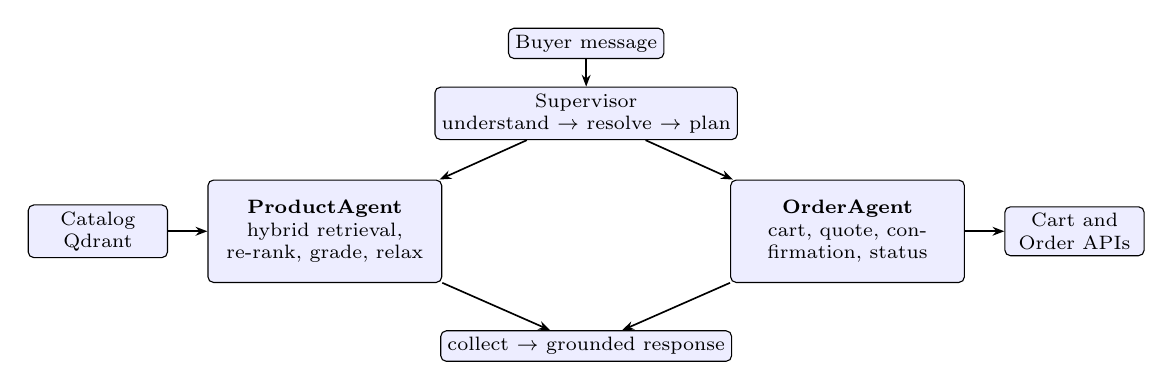
\begin{tikzpicture}[font=\scriptsize,
  box/.style={draw, rounded corners=2pt, fill=blue!7, align=center, inner sep=2.4pt},
  agent/.style={box, text width=28mm, minimum height=13mm},
  arr/.style={-{Stealth[length=1.5mm]}, semithick}]
\node[box] (msg) {Buyer message};
\node[box, below=3.5mm of msg] (sup) {Supervisor\\understand $\rightarrow$ resolve $\rightarrow$ plan};
\node[agent, below left=5mm and -1mm of sup] (prod) {\textbf{ProductAgent}\\hybrid retrieval, re-rank, grade, relax};
\node[agent, below right=5mm and -1mm of sup] (ord) {\textbf{OrderAgent}\\cart, quote, confirmation, status};
\node[box, below=6mm of $(prod.south)!0.5!(ord.south)$] (fin) {collect $\rightarrow$ grounded response};
\node[box, left=5mm of prod, text width=16mm] (cat) {Catalog\\Qdrant};
\node[box, right=5mm of ord, text width=16mm] (svc) {Cart and\\Order APIs};
\draw[arr] (msg) -- (sup);
\draw[arr] (sup) -- (prod);
\draw[arr] (sup) -- (ord);
\draw[arr] (cat) -- (prod);
\draw[arr] (ord) -- (svc);
\draw[arr] (prod) -- (fin);
\draw[arr] (ord) -- (fin);
\end{tikzpicture}
}
\caption{Implemented multi-agent architecture. The LLM supplies semantic plans; only the OrderAgent's deterministic commit path can perform transactional writes.}
\label{fig:architecture}
\end{figure}

The \textbf{ProductAgent} handles everything that only reads product data. Each product is stored in Qdrant as a 768-dimensional dense embedding plus a BM25 sparse vector~\cite{qdrant,lee2025geminiembedding,robertson2009bm25}, and the dense and lexical result lists are merged with reciprocal rank fusion~\cite{cormack2009rrf}. A multilingual cross-encoder, run locally, re-ranks the candidates. If LLM grading is switched on, the model then checks a short list against needs the catalog fields cannot capture (``easy for an elderly user,'' for example). When nothing matches, the agent relaxes constraints a limited number of times and can fall back to web research on the product type. Prices and stock are fetched again from the marketplace services before anything is shown. This agent cannot write to the cart or create orders.

The \textbf{OrderAgent} covers the cart view, proposed cart changes, checkout, confirmation, and order status. The model only ever sees numbered lists of real cart lines or product variants, so its choice has to point at something that exists; it has no way to make up an identifier. Every transaction is preceded by authentication and role checks. The key design decision is that preparing an action and committing it are separate steps. Preparation stores a pending action and returns a summary to the buyer. Nothing is written at that point.

\subsection{Transaction Safety Controls}

Figure~\ref{fig:sequence} shows how the protocol applies one rule, \emph{plan with the model, commit with the code}, at three boundaries.

\textit{Layer 1---conversational confirmation.} Any proposed change is saved as a pending action with a 144-bit random identifier, the exact payload, a summary the buyer can read, and a 600-s expiry. The assistant commits only if the same authenticated session sends that identifier back. Short replies are matched against fixed lists of accept and cancel phrases. For longer replies the model is consulted, but its answer counts only when the reply opens with an explicit phrase that agrees with it. A separate finalizer deletes any sentence saying the cart or an order has changed unless a write tool actually reported that change. The pending state is cleared as soon as the action succeeds or is canceled.

\textit{Layer 2---single-use checkout quote.} The assistant offers direct checkout only if the buyer already has a saved address and pays by cash on delivery or bank transfer. In every other case it simply opens the normal checkout page. To build a quote, the order service normalizes the product lines, reads the current price and stock, checks the address and voucher, and sets a 600-s expiry. It hands back a 256-bit token exactly once and keeps only the token's SHA-256 digest. The token lives in the assistant server's pending state; the browser never sees it, and it never enters an LLM prompt. At confirmation the service checks the buyer, chat session, token, status, and expiry. A conditional database update then moves the quote from \code{open} or \code{failed} to \code{committing}, and only the request that wins this update continues. Just before the order is created, every line is normalized again, and the request is rejected if price, stock, or product data changed. The order call carries \code{Idempotency-Key: checkout:\{quoteId\}}, so replaying a committed quote returns the order that already exists. Wallet payment is refused until the buyer gives a separate one-time payment approval.

\textit{Layer 3---retry-safe payment.} Once the order exists, the payment services run a saga with unique debit references, inbox deduplication, and transactional outboxes~\cite{richardson2018microservices}. If payment fails, the order can be canceled and its stock released. This layer is part of the deployed system, but our experiments end at order creation, and we make no evaluated claim about the payment saga.

\begin{figure}[t]
\centering
\resizebox{\columnwidth}{!}{%
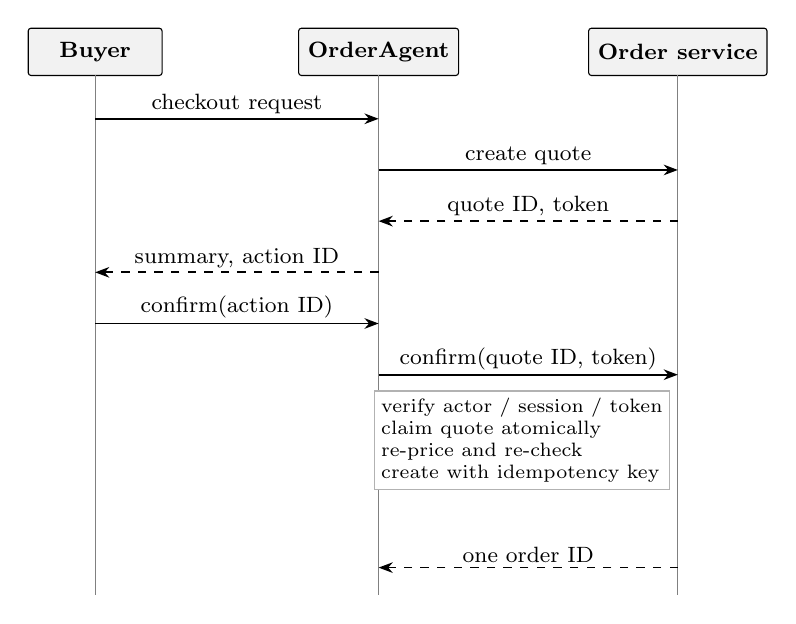
\begin{tikzpicture}[font=\footnotesize,
  life/.style={draw, fill=gray!10, rounded corners=1pt, minimum width=17mm, minimum height=6mm, font=\footnotesize\bfseries},
  msg/.style={-{Stealth[length=1.8mm]}, semithick}, ret/.style={-{Stealth[length=1.8mm]}, semithick, dashed},
  lbl/.style={above, inner sep=1.5pt}]
\def\xu{0}\def\xa{3.6}\def\xo{7.4}
\node[life] (u) at (\xu,0) {Buyer};
\node[life] (a) at (\xa,0) {OrderAgent};
\node[life] (o) at (\xo,0) {Order service};
\foreach \x in {\xu,\xa,\xo} \draw[gray] (\x,-0.3) -- (\x,-6.9);
\draw[msg] (\xu,-0.85) -- node[lbl]{checkout request} (\xa,-0.85);
\draw[msg] (\xa,-1.5) -- node[lbl]{create quote} (\xo,-1.5);
\draw[ret] (\xo,-2.15) -- node[lbl]{quote ID, token} (\xa,-2.15);
\draw[ret] (\xa,-2.8) -- node[lbl]{summary, action ID} (\xu,-2.8);
\draw[msg] (\xu,-3.45) -- node[lbl]{confirm(action ID)} (\xa,-3.45);
\draw[msg] (\xa,-4.1) -- node[lbl]{confirm(quote ID, token)} (\xo,-4.1);
\node[draw=gray!60, fill=white, align=left, anchor=north east, font=\scriptsize, inner sep=2.5pt] at (\xo-0.1,-4.3)
  {verify actor / session / token\\claim quote atomically\\re-price and re-check\\create with idempotency key};
\draw[ret] (\xo,-6.55) -- node[lbl]{one order ID} (\xa,-6.55);
\end{tikzpicture}%
}
\caption{Binding a conversational action to a server-side quote. The token remains between the assistant server and order service.}
\label{fig:sequence}
\end{figure}

\subsection{Experimental Design}

We wanted to test the commit path without also testing how well a model understands Vietnamese. The test programs therefore import the real agent graph, the OrderAgent, the confirmation functions, and the Node.js checkout controller, but swap out the LLM: E1 and E2 use a scripted semantic model, and E3 uses a classifier with controlled noise. Network services and storage are replaced by in-memory doubles that log every write. Faults can then be injected and repeated exactly. The price is that production latency and database isolation are not reproduced.

The four experiments are summarized in Table~\ref{tab:experiments}. E1 checks that conversations finish and that nothing is written too early. E2 injects faults one by one: authentication, identity, expiry, replay, price, concurrency, model, and downstream-service failures. E3 compares five authorization policies on 46 Vietnamese replies that we wrote and labeled ourselves (18 confirmations, 10 cancellations, and 18 replies of other kinds). Given an error probability $p$, the noisy model returns the true label with probability $1-p$ and otherwise picks one of the two wrong labels at random. We ran 2,000 trials for each $p\in\{0,.1,.2,.3,.4,.5\}$. E4 removes, in the service double, the quote claim, the idempotency key, both, or the re-pricing step.

\begin{table*}[t]
\caption{Evaluation Plan for the Single Research Question}
\label{tab:experiments}
\centering
\footnotesize
\setlength{\tabcolsep}{4pt}
\begin{tabular}{@{}p{17mm}p{48mm}p{68mm}p{35mm}@{}}
\toprule
Experiment & Input & Intervention and procedure & Measures \\
\midrule
E1 conversation & 200 direct and 200 checkout-page-handoff dialogues & Run the real graph with correct scripted semantic turns; inspect the recorded cart/order writes after each turn & Completion, early writes, orders, model calls, code time \\
E2 faults & 11 agent cases, 12 service cases, 7 response sentences & Inject one fault at a time, including forged/replayed IDs, expiry, price drift, unavailable model, retry, and 2/10/50 concurrent requests & Writes, orders, HTTP status, false success claims \\
E3 policies & 46 labeled replies; 2,000 trials per noise level & Compare direct action (V0), model only (V1), lexical only (V2), proposed two-stage gate (V3), and an in-sample refinement (V4) & False-confirm rate, confirmation recall, model calls \\
E4 guard removal & One quote under concurrency, lost response/retry, and price change & Remove atomic claim, idempotency key, both, or pre-commit re-pricing & Total and stale-price orders \\
\bottomrule
\end{tabular}
\end{table*}

For non-confirming replies $N$ and actual confirmations $Y$, let $FP_N$ be non-confirmations classified as confirm and $TP_Y$ be correctly accepted confirmations. The principal E3 metrics are
\begin{equation}
\mathrm{FCR}=\frac{FP_N}{|N|},\qquad
\mathrm{Recall}=\frac{TP_Y}{|Y|}.
\end{equation}
A lower false-confirm rate (FCR) means a safer system, and a higher recall means fewer annoyed buyers.

\subsection{Test Environment}

All experiments ran on one laptop, configured as in Table~\ref{tab:env}. No LLM API was called during the benchmarks, and no external service was contacted, so the results do not depend on network conditions or on a particular model provider. On the same commit, the assistant's own test suite passed 191 of 191 tests before the benchmarks were run. The benchmark scripts, the utterances, and the raw JSON results are in \code{docs/paper/benchmark}.

\begin{table}[t]
\caption{Hardware and Software Used for the Experiments}
\label{tab:env}
\centering
\footnotesize
\setlength{\tabcolsep}{4pt}
\begin{tabular}{@{}p{20mm}p{60mm}@{}}
\toprule
Component & Configuration \\
\midrule
Machine & ASUS ROG Zephyrus G14 (GA402RK) laptop \\
CPU & AMD Ryzen 9 6900HS, 8 cores / 16 threads \\
Memory & 32 GB RAM (31.2 GB usable) \\
GPU & AMD Radeon RX 6800S (discrete); Radeon integrated \\
Storage & 1 TB NVMe SSD (WD PC SN735) \\
OS & Windows 11 Home, build 26300 \\
Runtime & Python 3.10.0; Node.js 24.5.0 \\
Agent framework & LangGraph with in-memory checkpointer (\code{MemorySaver}) \\
LLM & Replaced by scripted / noisy doubles (no API calls) \\
Random seed & 20261108 (E3 noise model) \\
\bottomrule
\end{tabular}
\end{table}

\subsection{Synthetic Test Data}

The evaluation uses only synthetic data; no buyer conversations, orders, or personal data from the live marketplace were used. None of the test data was generated by an LLM or another AI tool. The data come from four sources.

\textit{Scripted dialogues (E1).} The 400 conversations are produced by the benchmark script from a fixed template: 200 in direct-checkout mode (four buyer messages each) and 200 in checkout-page-handoff mode (three messages each). Every run uses the same fixture of one catalog product (a white shirt), one stored delivery address, and an authenticated buyer. For each message, the script supplies the correct semantic turn that a perfect model would return, so E1 isolates the commit path from language understanding.

\textit{Fault cases (E2, E4).} The 11 agent-level cases, 12 order-service cases, and 7 response-filter sentences were written by hand, one per fault. Each case states its injected fault and its expected outcome (number of writes, number of orders, or HTTP status) before the run.

\textit{Labeled replies (E3).} The 46 Vietnamese replies to a pending action were written and labeled by the authors to cover common short confirmations (e.g., ``ok,'' ``close the order''), cancellations, and harder cases such as questions, hedges (``ok, but let me see another model first''), and replies that mix confirmation with a question. The label set has 18 confirmations, 10 cancellations, and 18 other replies.

\textit{Simulated model errors (E3).} Interpretation errors are not taken from a real LLM. A pseudo-random generator with seed 20261108 flips the gold label with probability $p$, picking one of the two wrong labels uniformly. A further worst-case model always answers ``confirm.'' Because the seed is fixed, rerunning the script reproduces the reported numbers exactly.

% ===========================================================================
\section{Experiments and Results}
\label{sec:results}

\subsection{Conversation Completion and Fault Injection}

Every one of the 400 E1 conversations ended where it was supposed to (Table~\ref{tab:e1}). In direct mode the assistant added a cart line and then placed one order, each step after its own confirmation. In handoff mode it added the line after confirmation and opened a pre-filled checkout page, leaving the final click to the normal interface. In no run was the cart changed or an order created ahead of time. Confirmations typed as fixed phrases never needed an LLM call. The median orchestration time was 5.9--8.1~ms per message. Because model, network, and database latency are not included, this figure reflects only the overhead of our code.

\begin{table}[t]
\caption{E1: Complete Checkout Conversations}
\label{tab:e1}
\centering
\footnotesize
\setlength{\tabcolsep}{4pt}
\begin{tabular}{@{}lcc@{}}
\toprule
Measure & Direct & Handoff \\
\midrule
Runs / messages per run & 200 / 4 & 200 / 3 \\
Goal reached & 200 & 200 \\
Writes / orders before confirmation & 0 / 0 & 0 / 0 \\
Cart writes / orders per run & 1 / 1 & 1 / 0 \\
LLM calls by turn & 1, 0, 1, 0 & 1, 0, 1 \\
Median code time (ms) & 8.1, 6.4, 7.6, 6.4 & 7.4, 5.9, 6.9 \\
\bottomrule
\end{tabular}
\end{table}

All 23 E2 fault cases gave the expected write count or status. On the agent side, a missing, forged, mismatched, expired, canceled, or unauthenticated action wrote nothing, and a replayed one wrote once. The explicit-prefix gate also turned down a hedged reply that the model had labeled as a confirmation. When the semantic model itself failed, the fallback path wrote nothing. Of the seven test sentences for the response filter, it removed all four unsupported ``done'' claims and kept the three factual or non-committal ones.

On the order-service side, a wrong token or session was rejected, an expired quote returned HTTP 410, a price change returned 409, and automatic wallet payment asked for step-up approval. A downstream order call that failed and was then retried produced one order. In the controller test double, batches of 2, 10, and 50 simultaneous confirmation calls each produced a single order. These runs check the conditional-claim logic; they say nothing about how a live database handles isolation.

\subsection{Confirmation-Policy Comparison}

As Fig.~\ref{fig:noise} shows, model-only authorization gets worse roughly in step with the injected error. V3 holds up better because the model's verdict is used only for replies whose wording already points to an explicit decision. At $p=0.3$, V1 accepted 15.1\% of non-confirmations and caught 70.2\% of real confirmations. V3 brought FCR down to 1.0\% and recall up to 91.8\%, calling the model 0.57 times per reply on average. The purely lexical V2 never confirmed falsely, but its recall stayed at 72.2\% because it threw out longer replies that were in fact valid.

\begin{figure*}[t]
\centering
\pgfplotsset{e3/.style={scale only axis, width=6.2cm, height=3.25cm, xmin=0, xmax=0.5,
  xtick={0,0.1,0.2,0.3,0.4,0.5}, tick label style={font=\footnotesize}, label style={font=\footnotesize},
  legend style={font=\footnotesize, at={(0.5,1.04)}, anchor=south, draw=none, legend columns=-1},
  every axis plot/.append style={thick, mark size=1.6pt}}}
\begin{tikzpicture}
\begin{axis}[e3, ymin=0, ymax=27, xlabel={Synthetic model error $p$}, ylabel={False confirmation (\%)}]
\addplot[red, mark=square*] coordinates {(0,0) (.1,4.9) (.2,9.9) (.3,15.1) (.4,19.8) (.5,25.1)};
\addplot[blue, mark=*] coordinates {(0,0) (.1,.3) (.2,.6) (.3,1.0) (.4,1.4) (.5,1.8)};
\addplot[black!60!green, mark=triangle*, dashed] coordinates {(0,0) (.1,0) (.2,0) (.3,0) (.4,0) (.5,0)};
\legend{V1 model-only,V3 proposed,V2 lexical}
\end{axis}
\end{tikzpicture}\hspace{9mm}%
\begin{tikzpicture}
\begin{axis}[e3, ymin=45, ymax=102, xlabel={Synthetic model error $p$}, ylabel={Confirmation recall (\%)}]
\addplot[red, mark=square*] coordinates {(0,100) (.1,89.8) (.2,80.0) (.3,70.2) (.4,60.1) (.5,49.5)};
\addplot[blue, mark=*] coordinates {(0,100) (.1,97.3) (.2,94.5) (.3,91.8) (.4,89.0) (.5,86.1)};
\addplot[black!60!green, mark=triangle*, dashed] coordinates {(0,72.2) (.1,72.2) (.2,72.2) (.3,72.2) (.4,72.2) (.5,72.2)};
\legend{V1 model-only,V3 proposed,V2 lexical}
\end{axis}
\end{tikzpicture}
\caption{E3 safety and convenience under controlled semantic-label noise. V0 is omitted because its false-confirm rate is 100\%.}
\label{fig:noise}
\end{figure*}

We also tried a worst-case classifier that answers ``confirm'' to everything. V1 then committed every reply. V3 still turned down 26 of the 28 non-confirmations; the two it let through were hedged replies starting with ``ok,'' which gives 7.1\% FCR. V4 adds three Vietnamese markers of contrast or deferral (the Vietnamese equivalents of ``but,'' ``let me \ldots\ first,'' and ``think it over''), and with them it rejected both replies at no cost to worst-case recall. We should be clear that V4 was built by looking at these same 46 utterances. It is a hypothesis to test on held-out data, not proof that the error rate is zero in general.

\subsection{Guard-Removal Results}

Table~\ref{tab:ablation} shows what each server-side guard contributes. Taking away only the claim, or only the key, did not lead to duplicate orders under concurrency in this double, since the guard that remained still merged the calls. With both gone, every concurrent request created its own order. The lost-response case is different: the service had created the order but the reply never arrived, and only the idempotency key stopped the retry from creating a second one. Likewise, only re-pricing caught an order whose catalog price had changed after the quote. The guards overlap in places but are not interchangeable. The claim decides which request owns a quote at a given moment, the key carries across downstream retries, and re-pricing ties the buyer's approval to the current state of the catalog.

\begin{table}[t]
\caption{E4: Orders After Removing a Guard}
\label{tab:ablation}
\centering
\footnotesize
\setlength{\tabcolsep}{3.5pt}
\begin{tabular}{@{}lccc@{}}
\toprule
Version & Concurrent 2/10/50 & Retry & Stale price \\
\midrule
Full protocol & 1 / 1 / 1 & 1 & 0 \\
No atomic claim & 1 / 1 / 1 & 1 & 0 \\
No idempotency key & 1 / 1 / 1 & \textbf{2} & 0 \\
No claim or key & \textbf{2 / 10 / 50} & \textbf{2} & 0 \\
No re-pricing & 1 / 1 / 1 & 1 & \textbf{1} \\
\bottomrule
\end{tabular}
\end{table}

\subsection{Answer to the Research Question}

Inside the commit boundary we tested, the architecture automated both direct checkout and handoff to the checkout page with no early writes. It contained the injected faults (identity, expiry, replay, retry, concurrency, price, and model failures), and it relied far less on the model to decide whether the buyer had agreed. Two results carry most of the weight. One is the drop in FCR from 15.1\% to 1.0\% at $p=0.3$, achieved alongside higher recall. The other is the ablation: duplicate and stale-price orders come back as soon as the matching guard is removed. Our answer is a qualified yes. The transaction safety controls worked in this implementation and under this test setup, but we cannot yet claim it holds at production scale or for real user populations.

% ===========================================================================
\section{Discussion}

\subsection{Implications}

The lesson we take from this work is to keep authority apart from interpretation. An LLM is good at turning a Vietnamese sentence into a structured choice, at resolving references, and at weighing fuzzy preferences. It should not have the last word on a write. To commit, the system should demand things a model cannot make up: an authenticated user, a pending action that the server created, the exact identifier, a token that has not expired, and the current state of the marketplace. A side benefit is that problems become easier to locate. The false-confirmation metric tells us about the conversational gate, and the concurrency and retry tests tell us about the service protocol, rather than both being folded into one end-to-end success rate.

The two agents differ in what they are allowed to do, not just in their names. The ProductAgent can only retrieve and read, and the OrderAgent is the one place where transactional state is prepared. Compared with giving every agent the same generic tools, this leaves much less to audit. Making the checkout-page handoff the default is a safety choice too. Direct checkout inside the chat is a shortcut, and it is offered only when the address and payment conditions are already met.

\subsection{Limitations and Threats to Validity}

\textbf{Construct validity.} Because E1 and E2 use scripted semantic turns, they test whether commits are correct, not whether the system understands free-form Vietnamese. E3 assumes label errors are independent, whereas real model errors cluster by phrasing, context, and model family. We wrote and labeled the 46 replies ourselves, and V4 was tuned on the same set.

\textbf{Internal validity.} The scripts load the production graph and controller but replace the databases and remote services. In the concurrency double the conditional update is atomic by construction, so a real deployment still needs an integration test against the configured database and its isolation level. Timings leave out model, network, and storage latency. The switches used in the ablation exist only in the service double, so the unsafe variants never reach production.

\textbf{External validity.} All results come from a single Vietnamese marketplace. Other languages, payment regulations, or user groups may behave differently. The study involved no human participants and no personal data, and we did not run a usability study. Search relevance, resistance to prompt injection, and the payment saga each need their own measurement. Next, we plan to test V3 and V4 on held-out replies collected from real users, run a real LLM against simulated buyers, repeat the concurrency and crash-recovery tests on databases configured as in production, and measure catalog retrieval on labeled Vietnamese queries.

% ===========================================================================
\section{Conclusion}

We set out to learn whether a multi-agent agentic RAG assistant can automate checkout without letting a probabilistic reading of the buyer's words authorize an unsafe order. In our architecture the ProductAgent reasons about the catalog and the OrderAgent prepares transactions, while the final decision belongs to deterministic confirmation, quote, re-pricing, and idempotency checks. In the code-level experiments, 400 conversations finished with no early writes and all 23 injected faults ended safely as expected. At 30\% synthetic model error, the confirmation gate cut false confirmations from 15.1\% to 1.0\% and improved recall at the same time. Removing guards one at a time showed that the atomic claim, the idempotency key, and the price re-check each do work the others cannot. For agents that move money, our practical advice is to let the model interpret and plan, but to commit only on evidence that the code itself holds.

% ===========================================================================


% ===========================================================================
\begin{thebibliography}{00}
\bibitem{lewis2020rag} P. Lewis, E. Perez, A. Piktus, F. Petroni, V. Karpukhin, N. Goyal, H. K\"{u}ttler, M. Lewis, W.-t. Yih, T. Rockt\"{a}schel, S. Riedel, and D. Kiela, ``\href{https://arxiv.org/abs/2005.11401}{Retrieval-augmented generation for knowledge-intensive NLP tasks},'' in \textit{Proc. Adv. Neural Inf. Process. Syst. (NeurIPS)}, vol. 33, 2020.
\bibitem{gao2023ragsurvey} Y. Gao, Y. Xiong, X. Gao, K. Jia, J. Pan, Y. Bi, Y. Dai, J. Sun, M. Wang, and H. Wang, ``\href{https://arxiv.org/abs/2312.10997}{Retrieval-augmented generation for large language models: A survey},'' 2023, arXiv:2312.10997.
\bibitem{singh2025agenticrag} A. Singh, A. Ehtesham, S. Kumar, T. T. Khoei, and A. V. Vasilakos, ``\href{https://arxiv.org/abs/2501.09136}{Agentic retrieval-augmented generation: A survey on agentic RAG},'' 2025, arXiv:2501.09136.
\bibitem{yao2023react} S. Yao, J. Zhao, D. Yu, N. Du, I. Shafran, K. Narasimhan, and Y. Cao, ``\href{https://arxiv.org/abs/2210.03629}{ReAct: Synergizing reasoning and acting in language models},'' in \textit{Proc. Int. Conf. Learn. Represent. (ICLR)}, 2023.
\bibitem{wu2023autogen} Q. Wu, G. Bansal, J. Zhang, \textit{et al.}, ``\href{https://arxiv.org/abs/2308.08155}{AutoGen: Enabling next-gen LLM applications via multi-agent conversation},'' 2023, arXiv:2308.08155.
\bibitem{yao2022webshop} S. Yao, H. Chen, J. Yang, and K. Narasimhan, ``\href{https://arxiv.org/abs/2207.01206}{WebShop: Towards scalable real-world web interaction with grounded language agents},'' in \textit{Proc. Adv. Neural Inf. Process. Syst. (NeurIPS)}, vol. 35, 2022.
\bibitem{yao2024taubench} S. Yao, N. Shinn, P. Razavi, and K. Narasimhan, ``\href{https://arxiv.org/abs/2406.12045}{$\tau$-bench: A benchmark for tool-agent-user interaction in real-world domains},'' 2024, arXiv:2406.12045.
\bibitem{greshake2023injection} K. Greshake, S. Abdelnabi, S. Mishra, C. Endres, T. Holz, and M. Fritz, ``\href{https://arxiv.org/abs/2302.12173}{Not what you've signed up for: Compromising real-world LLM-integrated applications with indirect prompt injection},'' in \textit{Proc. ACM Workshop Artif. Intell. Secur.}, 2023, pp. 79--90.
\bibitem{debenedetti2024agentdojo} E. Debenedetti, J. Zhang, M. Balunovi\'{c}, L. Beurer-Kellner, M. Fischer, and F. Tram\`{e}r, ``\href{https://arxiv.org/abs/2406.13352}{AgentDojo: A dynamic environment to evaluate prompt injection attacks and defenses for LLM agents},'' in \textit{Proc. NeurIPS Datasets Benchmarks Track}, 2024.
\bibitem{ruan2024toolemu} Y. Ruan, H. Dong, A. Wang, \textit{et al.}, ``\href{https://arxiv.org/abs/2309.15817}{Identifying the risks of LM agents with an LM-emulated sandbox},'' in \textit{Proc. Int. Conf. Learn. Represent. (ICLR)}, 2024.
\bibitem{garciamolina1987sagas} H. Garcia-Molina and K. Salem, ``\href{https://doi.org/10.1145/38713.38742}{Sagas},'' in \textit{Proc. ACM SIGMOD Int. Conf. Manage. Data}, 1987, pp. 249--259.
\bibitem{helland2012idempotence} P. Helland, ``Idempotence is not a medical condition,'' \textit{ACM Queue}, vol. 10, no. 4, p. 30, Apr. 2012.
\bibitem{richardson2018microservices} C. Richardson, \textit{Microservices Patterns: With Examples in Java}. Shelter Island, NY, USA: Manning, 2018.
\bibitem{kreps2011kafka} J. Kreps, N. Narkhede, and J. Rao, ``\href{https://course.ece.cmu.edu/~ece845/sp19/docs/kafka.pdf}{Kafka: A distributed messaging system for log processing},'' in \textit{Proc. 6th Int. Workshop Netw. Meets Databases}, 2011.
\bibitem{langgraph} LangChain, ``\href{https://github.com/langchain-ai/langgraph}{LangGraph: Build resilient language agents as graphs},'' Software. Accessed: Nov. 8, 2026.
\bibitem{qdrant} Qdrant, ``\href{https://github.com/qdrant/qdrant}{Qdrant: Vector search engine and vector database},'' Software. Accessed: Nov. 8, 2026.
\bibitem{lee2025geminiembedding} J. Lee, F. Chen, S. Dua, D. Cer, M. Shanbhogue, I. Naim, \textit{et al.}, ``\href{https://arxiv.org/abs/2503.07891}{Gemini Embedding: Generalizable embeddings from Gemini},'' 2025, arXiv:2503.07891.
\bibitem{robertson2009bm25} S. Robertson and H. Zaragoza, ``\href{https://doi.org/10.1561/1500000019}{The probabilistic relevance framework: BM25 and beyond},'' \textit{Found. Trends Inf. Retr.}, vol. 3, no. 4, pp. 333--389, 2009.
\bibitem{cormack2009rrf} G. V. Cormack, C. L. A. Clarke, and S. B\"{u}ttcher, ``Reciprocal rank fusion outperforms Condorcet and individual rank learning methods,'' in \textit{Proc. ACM SIGIR}, 2009, pp. 758--759.
\end{thebibliography}

\end{document}
